\begin{figure}
	\centering
	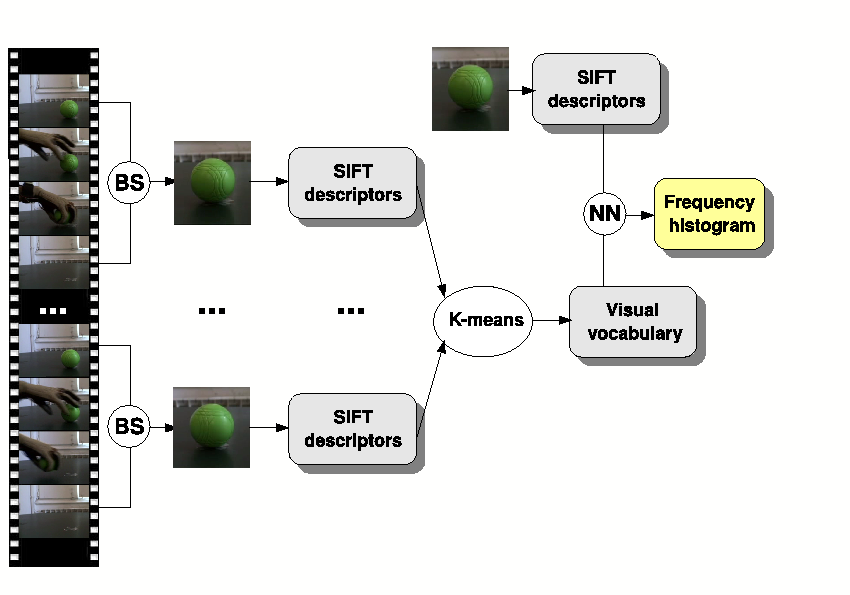
\includegraphics[width=0.8\textwidth]{images/schema_vision}
	\caption{A schema of the vision unit. First, suitable frames are extracted from the sequence and objects are located by means of background subtaction (BS). SIFT descriptors of a set of random points are input of a clustering step to get to the final visual vocabulary. Finally, each image is represented with respect to the vocabulary adopting a nearest neighbour (NN) strategy (see text for details).}
	\label{fig::vision}
\end{figure}

\section{Vision unit}
\label{sec::vision}
As we will discuss in Sec. \ref{sec::experiments}, the system gathers, as one input, a video sequence acting as {\it spectator}, whose focus is on object appearance. The goal of the vision unit is to process the signal to obtain a global model of a set of given objects.
Figure \ref{fig::vision} shows the pipeline of the vision unit when considering only one object (the same procedure is applied to the whole set of objects). Among the sequence, we first select the frames showing only the object  without any occlusion, then we locate more precisely its position by means of a simple background subtraction. 
Although in our application there is not an explicit object recognition step, it is clear from the architecture pipeline that a robust and specific object model is functional to subsequent analysis. It is worthwhile also to mention that with the terms {\it object recognition} we indicate the characterization of a specific object instance (againts the concept of categorizing classes of objects).
We adopt an approach based on local features to describe image structures: because of their popularity a rich variety of local measurements have been proposed in the literature \cite{harris,schmid,lowe} and applied successfully to objects recognition and categorization problems (see \cite{csurka,ferrari} just to name a few). 
Local approaches tipically include two distinct steps: keypoints extraction and description. 
However, in our case, a keypoint based-representation often ends up into a poor description
due to the limited size of the images. We thus built our representation by extracting enough 
random points  guaranteeing a more homogenous sampling.
We chose to adopt SIFT descriptors \cite{lowe,schmid2} to model image patches around these points, obtaining a set of {\it words} for each image.\\
To avoid redundancy and include some global information in our model, we apply k-means \cite{wong}, following the well-known bag-of-words approach \cite{csurka}. 
We thus build a {\it global} vocabulary, containing SIFT descriptions of all known objects. 
Image representation is obtained by means of frequency histogram of visual words, selecting for each random point extracted from the image 
the most similar visual word as nearest neighbor. A normalization step may be advisable for the subsequent data processing.